% !TeX root = ../main.tex
% Add the above to each chapter to make compiling the PDF easier in some editors.

\chapter{Implementation}\label{chapter:Implementation}
Subsequent chapter is going to give a detailed view on how the methods described in section \ref{chapter:Concept}, were implemented. Moreover possible problems regarding the process are listed. 
As i took the android-application described in passage \ref{chapter:Integration into existing App} as a basis, there is no reasonable alternative to further developing the app with Android Studio.

\section{Native Development Kit}
 The Android NDK is a toolset that lets you implement parts of your app in native code, using languages such as C and C++. For certain types of apps, this can help you reuse code libraries written in those languages \cite{androidndk}. Moreover employing the Native Development Kit to your Java code can increase the performance of the application significantly  \cite{ndkspeed}. I anticipated using the Native Kit might have a bigger workload, than Android's classic SDK, but I thought this to be alright, if the performance was superiorly compared to the approach written in Java. \newline
 First part, dealing with the detection of Speed Signs, doing image processing with OpenCV,  was relatively simple in C++, compared to the mammoth task of building Tensorflow from source, loading a model and integrating integrating everything into the actual app. It actually was so time consuming, I did not think I could manage to make it work on schedule. A lack of supporting features like Code Completion in Android Studio, poor documentation from Tensorflow (at least for average developers) paired with proportionally sparse discussion board entries like "Stack Overflow", that often referenced different versions, led me to the turning point, where I gave up using the NDK for the SDK. In total, this excursion cost me about one to two weeks of my time, reserved for implementation.  
 
\section{Extracting Speed Sign Candidates}
I implemented the algorithm in three languages: C++, Java and Python, every language serving different purposes. C++ and Java versions where necessary to operate for the application, first one running the Native approach, the second for the "standard" version. Last program written in Python was utilized for extracting data from images collected from Google image search, running on my PC, in order to get training data to feed my Neural Network model (more about this topic later on). Nevertheless, apart from syntactical differences, every program basically does the same operations. For the sake of simplicity I am only going to present the python variation, as it is probably the easiest to read.\newline
After reading the image, changing the colourspace from RGB/BGR to HSL/HSV is an optional, but reasonable step, because in the RGB/BGR space, all three Values of red, green and blue are correlated when it comes to changes in brightness \cite{imagesegmentation}. Unlike that, HSL/HSV holds lightness or the value of brightness in a separate variable, which can lead to better results with respect to filtering colours under difficult lighting conditions. In the following we are going to stick to the HSV space, even though both work almost analogical, they differentiate each other from the arrangement of brightness. \newline
Nevertheless filtering red pixels from our preferred colourspace works slightly different than just excerpting the Red channel of an image, as you would using RGB:
\begin{figure}[H]
	\minipage{\textwidth}
	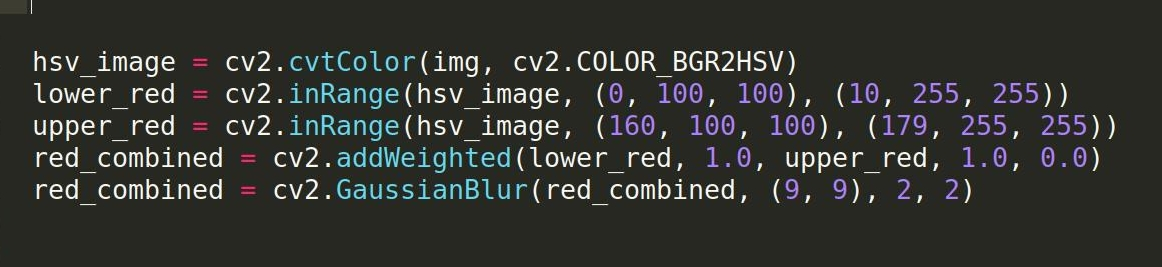
\includegraphics[width=\linewidth]{images/filterredimage.jpg}
	\caption{Python code for extracting red pixels}\label{fig:pythonredpix}
	\endminipage\hfill
\end{figure}

\begin{figure}[H]
	\centering
	\minipage{0.5\textwidth}
	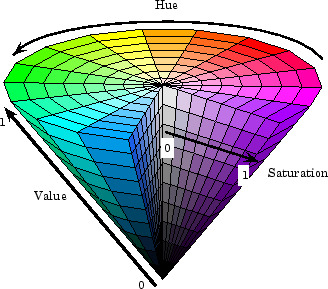
\includegraphics[width=\linewidth]{images/hsv.jpg}
	\caption{HSV colourspace}\label{fig:hsv}
	\endminipage\hfill
\end{figure}



\section{Neural Net Classification}
\subsection{Building Neural Network}
